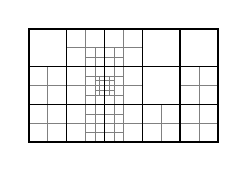
\begin{tikzpicture}[scale=0.12]

	\def\startx{0}
	\def\starty{0}
	\def\dimx{20}
	\def\dimy{-12}

	% first row
	\draw[step=2,help lines] (\startx+4,\starty) grid (\startx+8,\starty-2);
	\draw[step=1,help lines] (\startx+6,\starty-2) grid (\startx+8,\starty-4);

	\draw[step=2,help lines] (\startx+8,\starty) grid (\startx+12,\starty-4);
	\draw[step=1,help lines] (\startx+8,\starty-2) grid (\startx+10,\starty-4);
	
	% second row
	\draw[step=2,help lines] (\startx+0,\starty-4) grid (\startx+4,\starty-8);
	
	\draw[step=2,help lines] (\startx+4,\starty-4) grid (\startx+8,\starty-8);
	\draw[step=1,help lines] (\startx+6,\starty-4) grid (\startx+8,\starty-8);

	\draw[step=2,help lines] (\startx+8,\starty-4) grid (\startx+12,\starty-8);
	\draw[step=1,help lines] (\startx+8,\starty-4) grid (\startx+10,\starty-8);

	\draw[step=2,help lines] (\startx+16,\starty-4) grid (\startx+20,\starty-8);

	\draw[step=0.5,help lines] (\startx+7,\starty-5) grid (\startx+9,\starty-7);

	% third row
	\draw[step=2,help lines] (\startx+0,\starty-8) grid (\startx+20,\starty-12);
	\draw[step=1,help lines] (\startx+6,\starty-8) grid (\startx+10,\starty-12);

	% redraw the border
	\draw[step=4] (\startx,\starty) grid (\dimx,\dimy);
	\draw[thick] (\startx, \starty) rectangle (\dimx,\dimy);
\end{tikzpicture}

% vim:set filetype=tex:
